\section{Métodos computacionales}

\subsection{Protocolo de litiación}\label{s:litpro}

Se propone un protocolo de litiación, similar al que presentaron Chevrier y Dahn
\cite{chevrier2009} que se utilizó en la sección \ref{s:dftcalc}, que consiste 
en los siguientes pasos:
\begin{enumerate}
    \item Agregar un átomo de Li en el centro de la esfera vacía más grande que se pueda definir en el sistema.
        Para encontrar dicho punto se calculan los centros de la triangulación 
        de Delaunay, que se corresponden a los vértices de un diagrama de 
        Voronoi \cite{aurenhammer1991}. Desde estos puntos se computa la 
        distancia al átomo más cercano y se selecciona como centro aquel que 
        tenga la mayor distancia. 
    \item Aumentar  el volumen y escalar las coordenadas por un factor para
        seguir la expansión experimental del sistema.
    \item Minimizar localmente las coordenadas, con el algoritmo LBFGS \cite{liu1989} en este caso.
    \item Correr una simulación de dinámica molecular en el ensamble $NPT$, en 
        este caso utilizando el termostato y el barostato de Berendsen \cite{berendsen1984} 
        disponibles en el código \path{DFTB+} \cite{dftb+} por 10 ps. 
    \item Seleccionar la estructura con menor presión absoluta.
    \item Si $x < 3.75$ se vuelve al paso 1 y sino se termina la litiación.
\end{enumerate}
El paso (4) representa una modificación ligera que mejora la optimización a 
cambio de volumen fijo como se realiza en la referencia \cite{chevrier2009}.
Partiendo de la estructura de silicio amorfo obtenida en la sección 
\ref{s:rdfb} y siguiendo este protocolo de litiación, se obtienen estructuras
amorfas para un rango amplio de concentraciones de Li en Li$_x$Si. Se comienza
con los 64 átomos de Si iniciales ($x=0$) y se llega a un total de 304 átomos
para la estructura completamente litiada ($x=3.75$). Todos los observables que
se presentan a continuación para cada valor particular de $x$ se calcularon 
utilizando una trayectoria más larga de 0.5 ns. Los valores optimizados de $x$
son $0.20, 0.56, 0.89, 1.50, 2.00, 2.50, 3.28, 3.75$. Estas estructuras se 
muestran en la Figura \ref{fig:litiacion} y, además, fueron publicadas en un 
repositorio de libre acceso \cite{dftb_lisi_amorphous}.
\begin{figure}[h!]
    \centering
    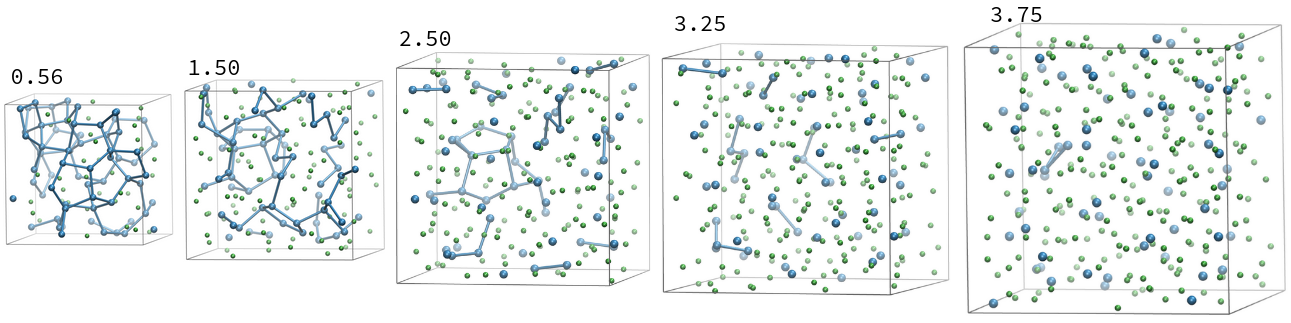
\includegraphics[width=\textwidth]{Silicio/prediccion/metodos/litiacion.png}
    \caption{Estructuras amorfas de Li$_x$Si obtenidas con el protocolo de litiación
    propuesto para distintos valores de $x$ (etiqutas de cada estructura). Los 
    átomos de Si se muestran en azul, los de Li en verde y la celda periódica en 
    gris. Los enlaces Si-Si están graficados si la distancia entre los mismos es
    menor a 3.0 \AA. Las estructuras no se encuentran a escala entre sí.}
    \label{fig:litiacion}
\end{figure}
